\documentclass[aspectratio=169,xcolor=dvipsnames, t]{beamer}

\usepackage{cp24}
\usepackage[square,numbers]{natbib}

\bibliographystyle{ACM-Reference-Format}

%*************************************************************************************************************
\title[Customizable Roundtrips with Tour4Me]{Customizable Roundtrips with Tour4Me}
\subtitle{Meta-heuristic Approaches for Personalized Running and Cycling Routes}
\author[Lisa Salewsky]{
	Lisa Salewsky
}


\institute[TU Dortmund]{
	\begin{minipage}[t][2.3cm][b]{0.7\textwidth}
		\centering
		\begin{tikzpicture}[remember picture,overlay]
			\node[inner sep=0] at (2.5,-0.8) {
\includegraphics[scale=0.1]{logo.png}};
		\end{tikzpicture}
		TU Dortmund, Fakultät für Informatik\\
		\vspace{1.5cm}
		Reviewer:\\
		Prof. Dr. Kevin Buchin\\
		Mart Hagedoorn, M. Sc.
	\end{minipage}
	
}
\date[\today]{\today}
\beamertemplatenavigationsymbolsempty %Navigantionszeite unten aus
%*************************************************************************************************************
%\usetheme{Malmoe} 
%\usetheme{Madrid}
%\usecolortheme{rose} %schwache farben
% Themes:
%AnnArbor | Antibes | Bergen |Berkeley | Berlin | Boadilla |boxes | CambridgeUS | Copenhagen |Darmstadt | default | Dresden |
%Frankfurt | Goettingen |Hannover | Ilmenau | JuanLesPins | Luebeck | Madrid | Malmoe | Marburg |
%Montpellier | PaloAlto | Pittsburgh |Rochester | Singapore | Szeged |Warsaw
\useinnertheme{rounded}
%\useoutertheme{shadow} %schattierung in den Rechtecken der Blocken -- nix
%*************************************************************************************************************


% Customize the table of contents
\setbeamertemplate{section in toc}[square]
\setbeamertemplate{subsection in toc}[square]
\setbeamertemplate{section/subsection in toc}[square]
\setbeamercolor{section number projected}{bg=tu_green_full,fg=white}
\setbeamercolor{subsection number projected}{bg=tu_green_full,fg=white}

% Customize all the bulletpoints
\setbeamertemplate{items}[square]

% Customize the link colors
\hypersetup{
	colorlinks=true,
	linkcolor=tu_green_full2,
	urlcolor=tu_green_full2,
	citecolor=tu_green_full2
}

\setbeamercolor{block title}{bg=tu_light_green_full2, fg=black}
\setbeamercolor{block body}{bg=tu_light_green_full3, fg=black}


\begin{document}
	%*************************************************************
	\begin{frame}
		\thispagestyle{empty}
		\titlepage
	\end{frame}
	%*************************************************************
%	
%	\begin{frame}{Agenda}
%		\centering	
%		\tableofcontents
%	\end{frame}
	
	\section{Einleitung}
	
	\begin{frame}{Einleitung}
		\vspace{0.25cm}
		Warum eine App zum Erstellen von Rundrips?
		\only<2>{	
			\begin{figure}
				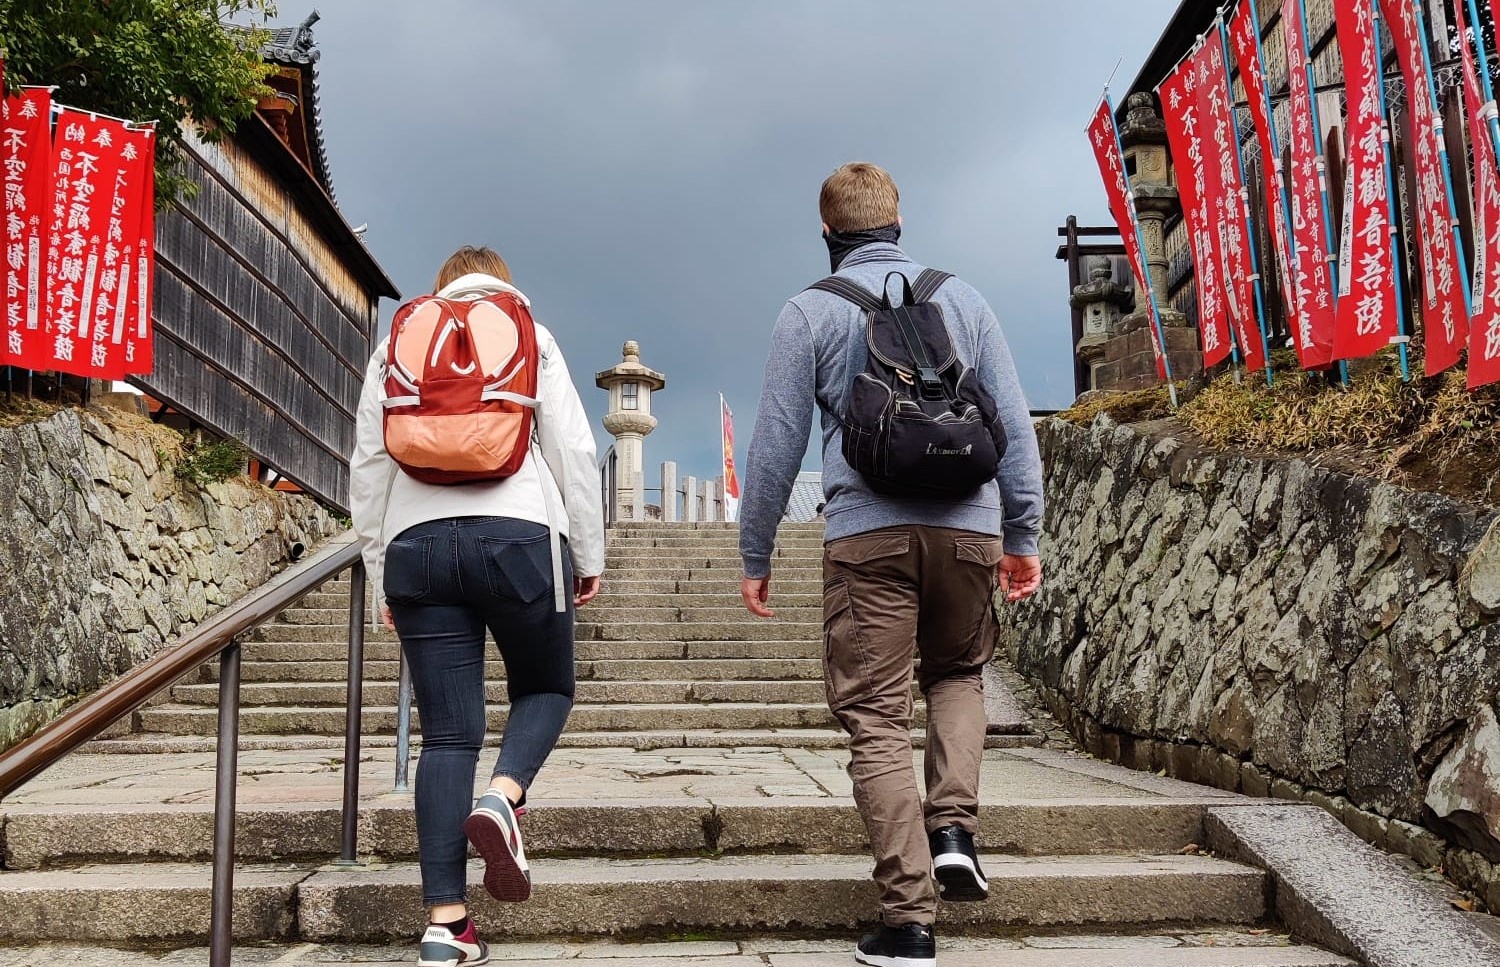
\includegraphics[height=0.6\textheight]{images/IMG-20231124-WA0010-cropped.jpg}
			\end{figure}}
		\only<3>{	
			\begin{figure}
				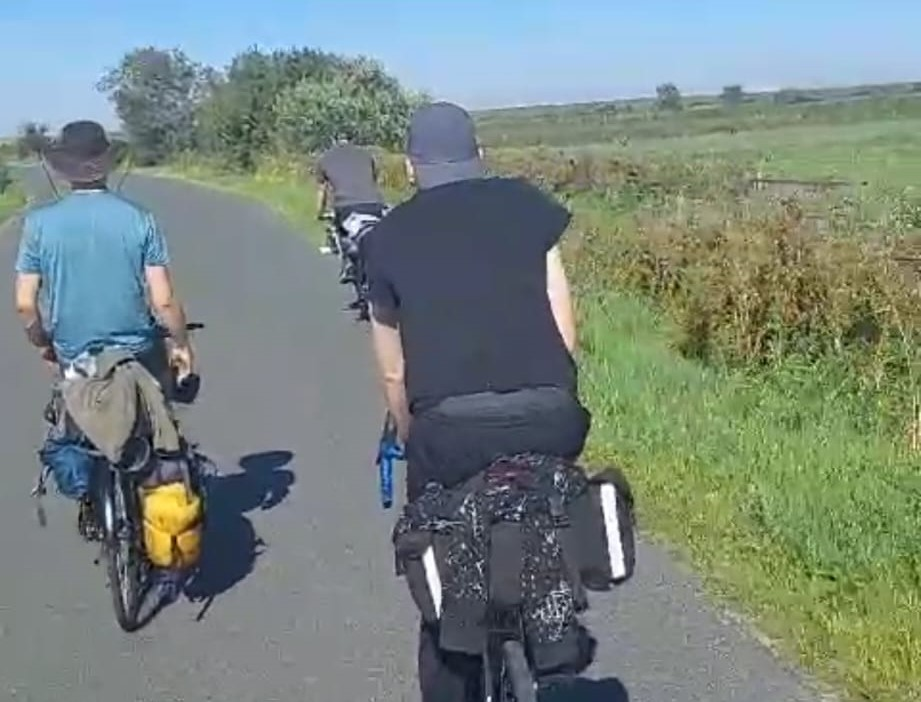
\includegraphics[height=0.6\textheight]{images/IMG-20231124-WA0039-cropped.jpg}
			\end{figure}}
		\only<4>{	
			\begin{figure}
				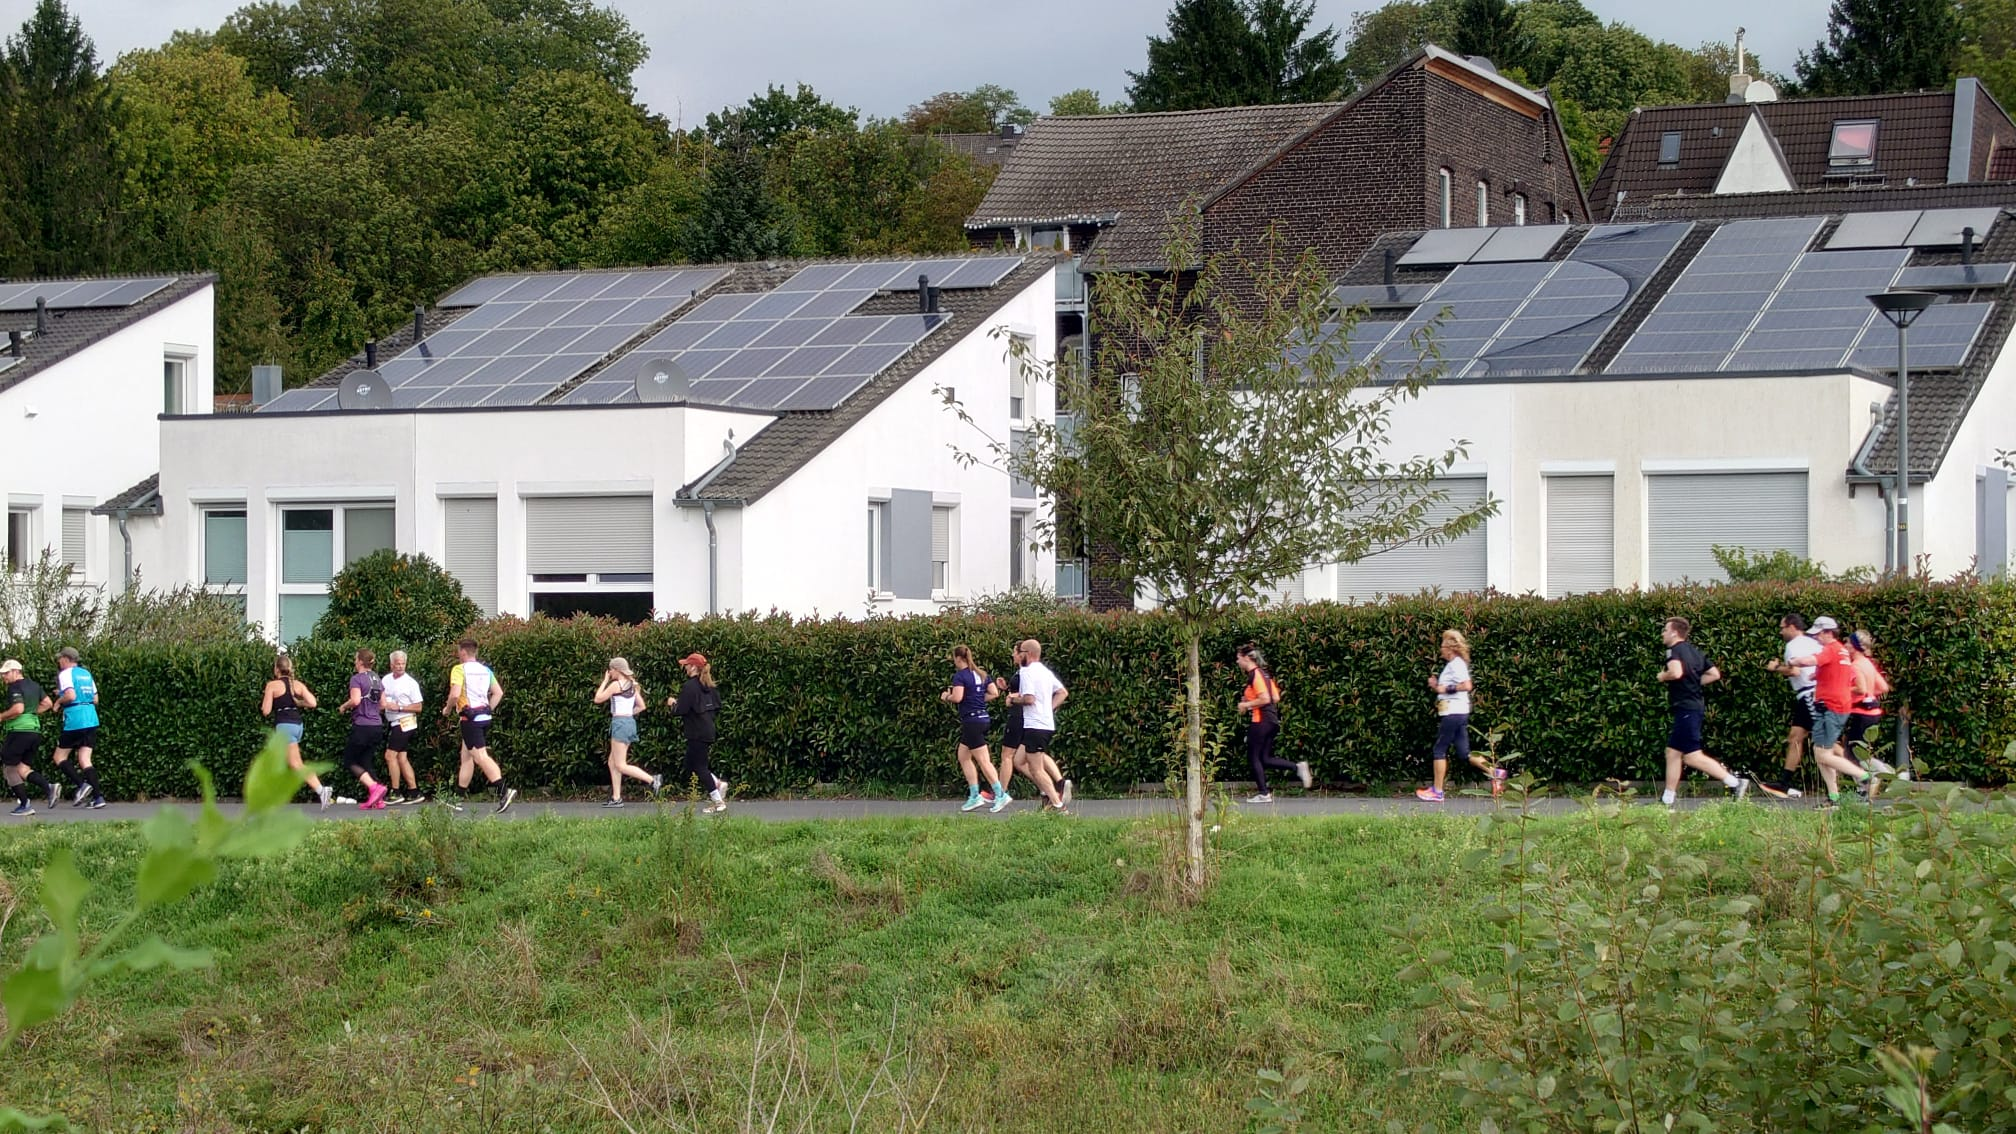
\includegraphics[height=0.6\textheight]{images/WhatsApp Bild 2023-11-24 um 14.35.53_5752c78a.jpg}
			\end{figure}}
	\end{frame}
	\begin{frame}{Einleitung}
		\vspace{0.25cm}
		Warum eine App zum Erstellen von Rundrips?
		\begin{columns}
			\begin{column}{0.48\textwidth}
				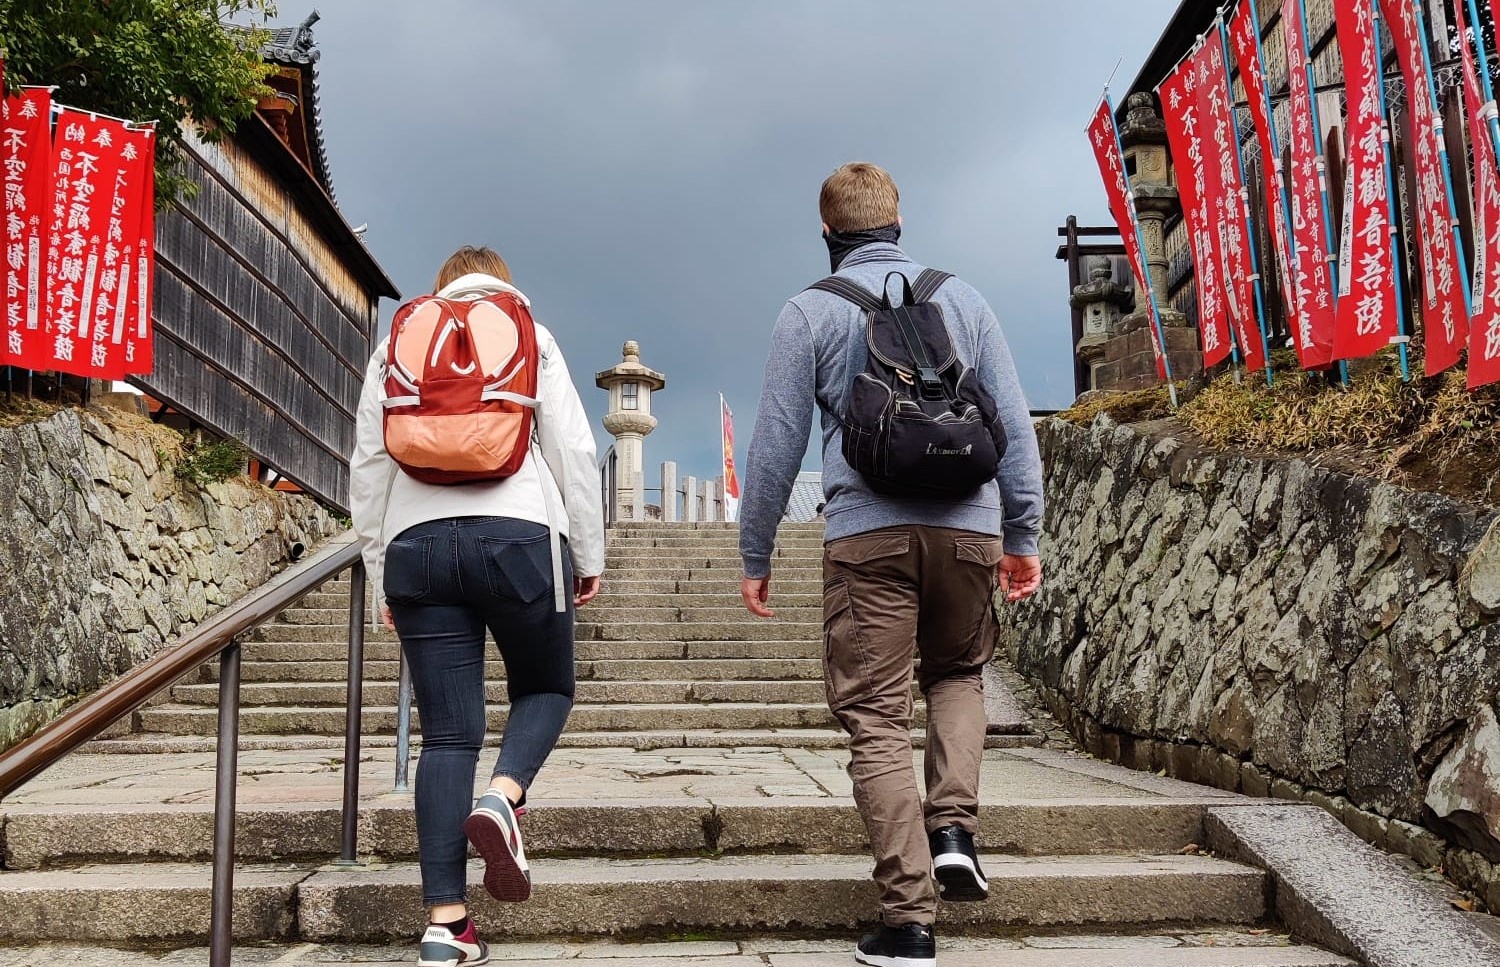
\includegraphics[height=0.3\textheight]{images/IMG-20231124-WA0010-cropped.jpg}
			\vspace{-1.5cm}
				\begin{flushright}
					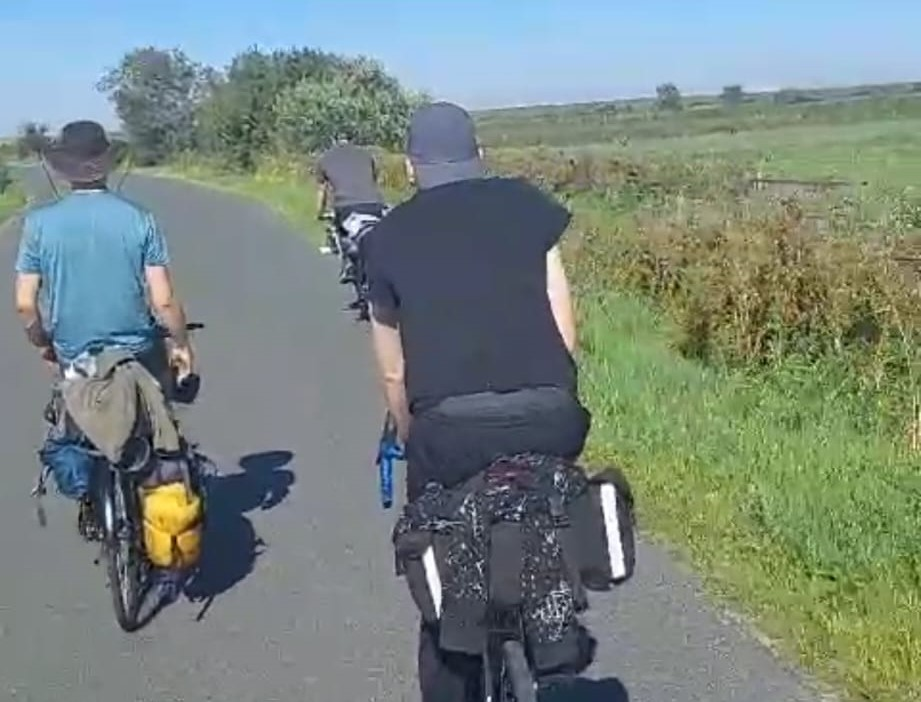
\includegraphics[height=0.3\textheight]{images/IMG-20231124-WA0039-cropped.jpg}
				\end{flushright}
			\vspace{-1cm}
				\begin{flushleft}
					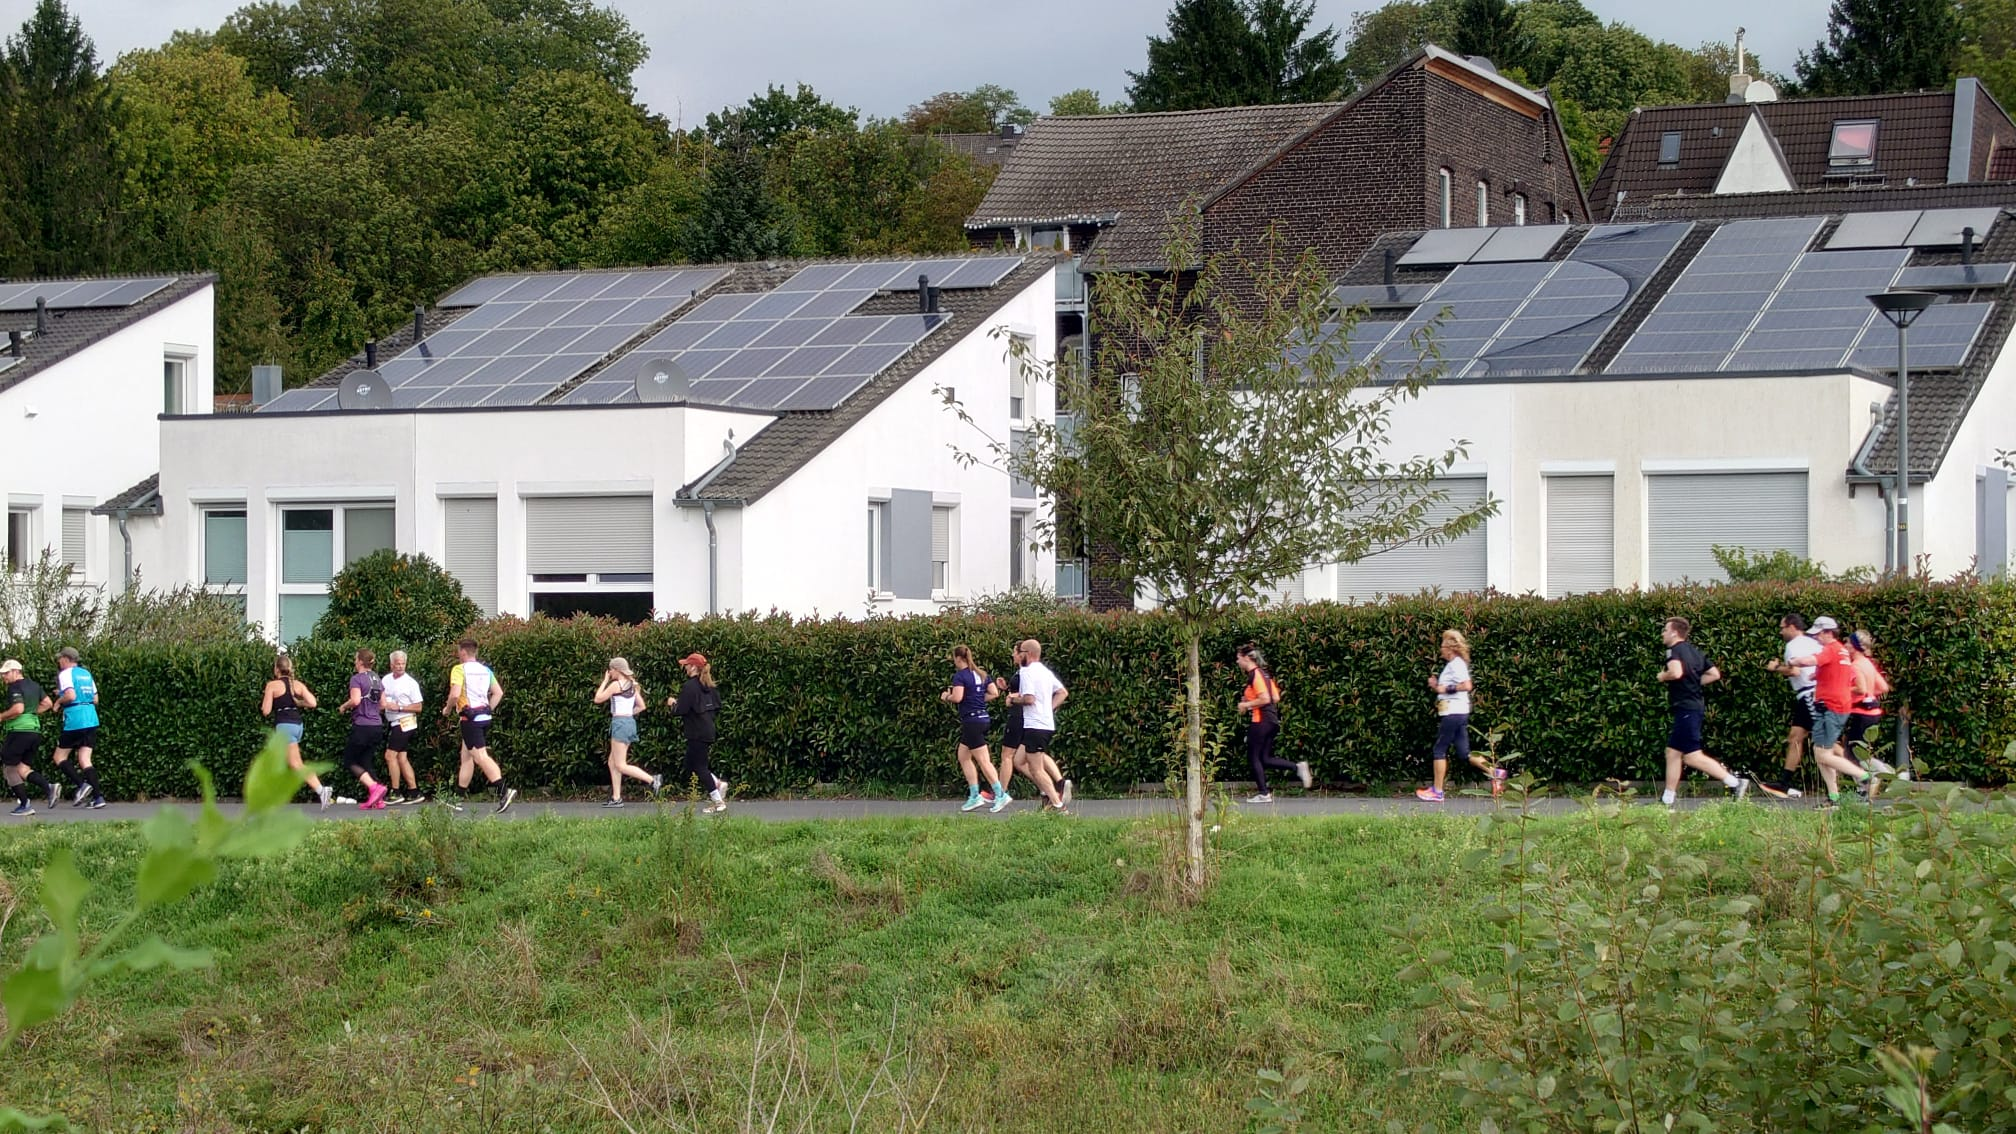
\includegraphics[height=0.3\textheight]{images/WhatsApp Bild 2023-11-24 um 14.35.53_5752c78a.jpg}
				\end{flushleft}
		\end{column}
		\begin{column}{0.48\textwidth}
			\vspace{-2cm}
			\begin{block}{Gemeinsamkeiten}
				\pause
				\begin{itemize}
					\only<2>{\item Trips von A nach B}
					\only<3->{\item Trips von A nach B?}
					\item<4-> In der Freizeit aber oft Rundtrips
					\item<5-> Möglichst "hübsche" Routen mit zusätzlichen individuellen Wünschen gewünscht
				\end{itemize}
			\end{block}
		\end{column}
		\end{columns} ~\\
		
	\end{frame}
	
	\begin{frame}{Einleitung}
	\vspace{0.25cm}
	Warum eine App zum Erstellen von Rundrips?
	\pause
	\begin{itemize}	
		\item<2-> Viele Lösungen für kürzeste Wege von A nach B
		\item<3-> Optimieren alltägliche Routen
		\item<4-> Joggen und Radfahren in der Freizeit:
		\item<5-> Weitere Bedingungen für attraktive Strecken nötig
		\only<6>{\item Aber kaum Ansätze für Rundtrips}
		\only<7->{\item Aber kaum Ansätze für Rundtrips mit Präferenzen}
	\end{itemize}
	\end{frame}

	\begin{frame}{Einleitung}
		\vspace{0.25cm}
		Was macht eine Strecke attraktiv?\\
		\pause
		\vspace{-0.2cm}
		\begin{minipage}[t]{0.48\textwidth}
			\begin{itemize}[<+->]
				\item Abhängig von individuellen Bedürfnissen und vom Level der Person
				\item Viele verschiedene Faktoren
				\begin{itemize}[<+->]
					\item Wegtyp (Straße, Waldpfad, Radweg etc.)
					\item Untergrund (Teer, Kies, Sand, Erde, etc.)
					\item Steigung
					\item Umgebung (Wald, Park, Wohngegend, etc.)
					\item Form (Rund, gerade mit U-Turn, viele Abzweigungen, etc.)
				\end{itemize}
				\item Einfluss dieser auf Strecke individuell auswählen 
		\end{itemize}
		\end{minipage}
		\begin{minipage}[t][0.7\textheight][b]{0.48\textwidth}
			\only<4>{
				\includegraphics[height=0.5\textheight]{images/IMG_20220921_181918.jpg}
				\vspace{-4cm}
				\begin{flushright}
					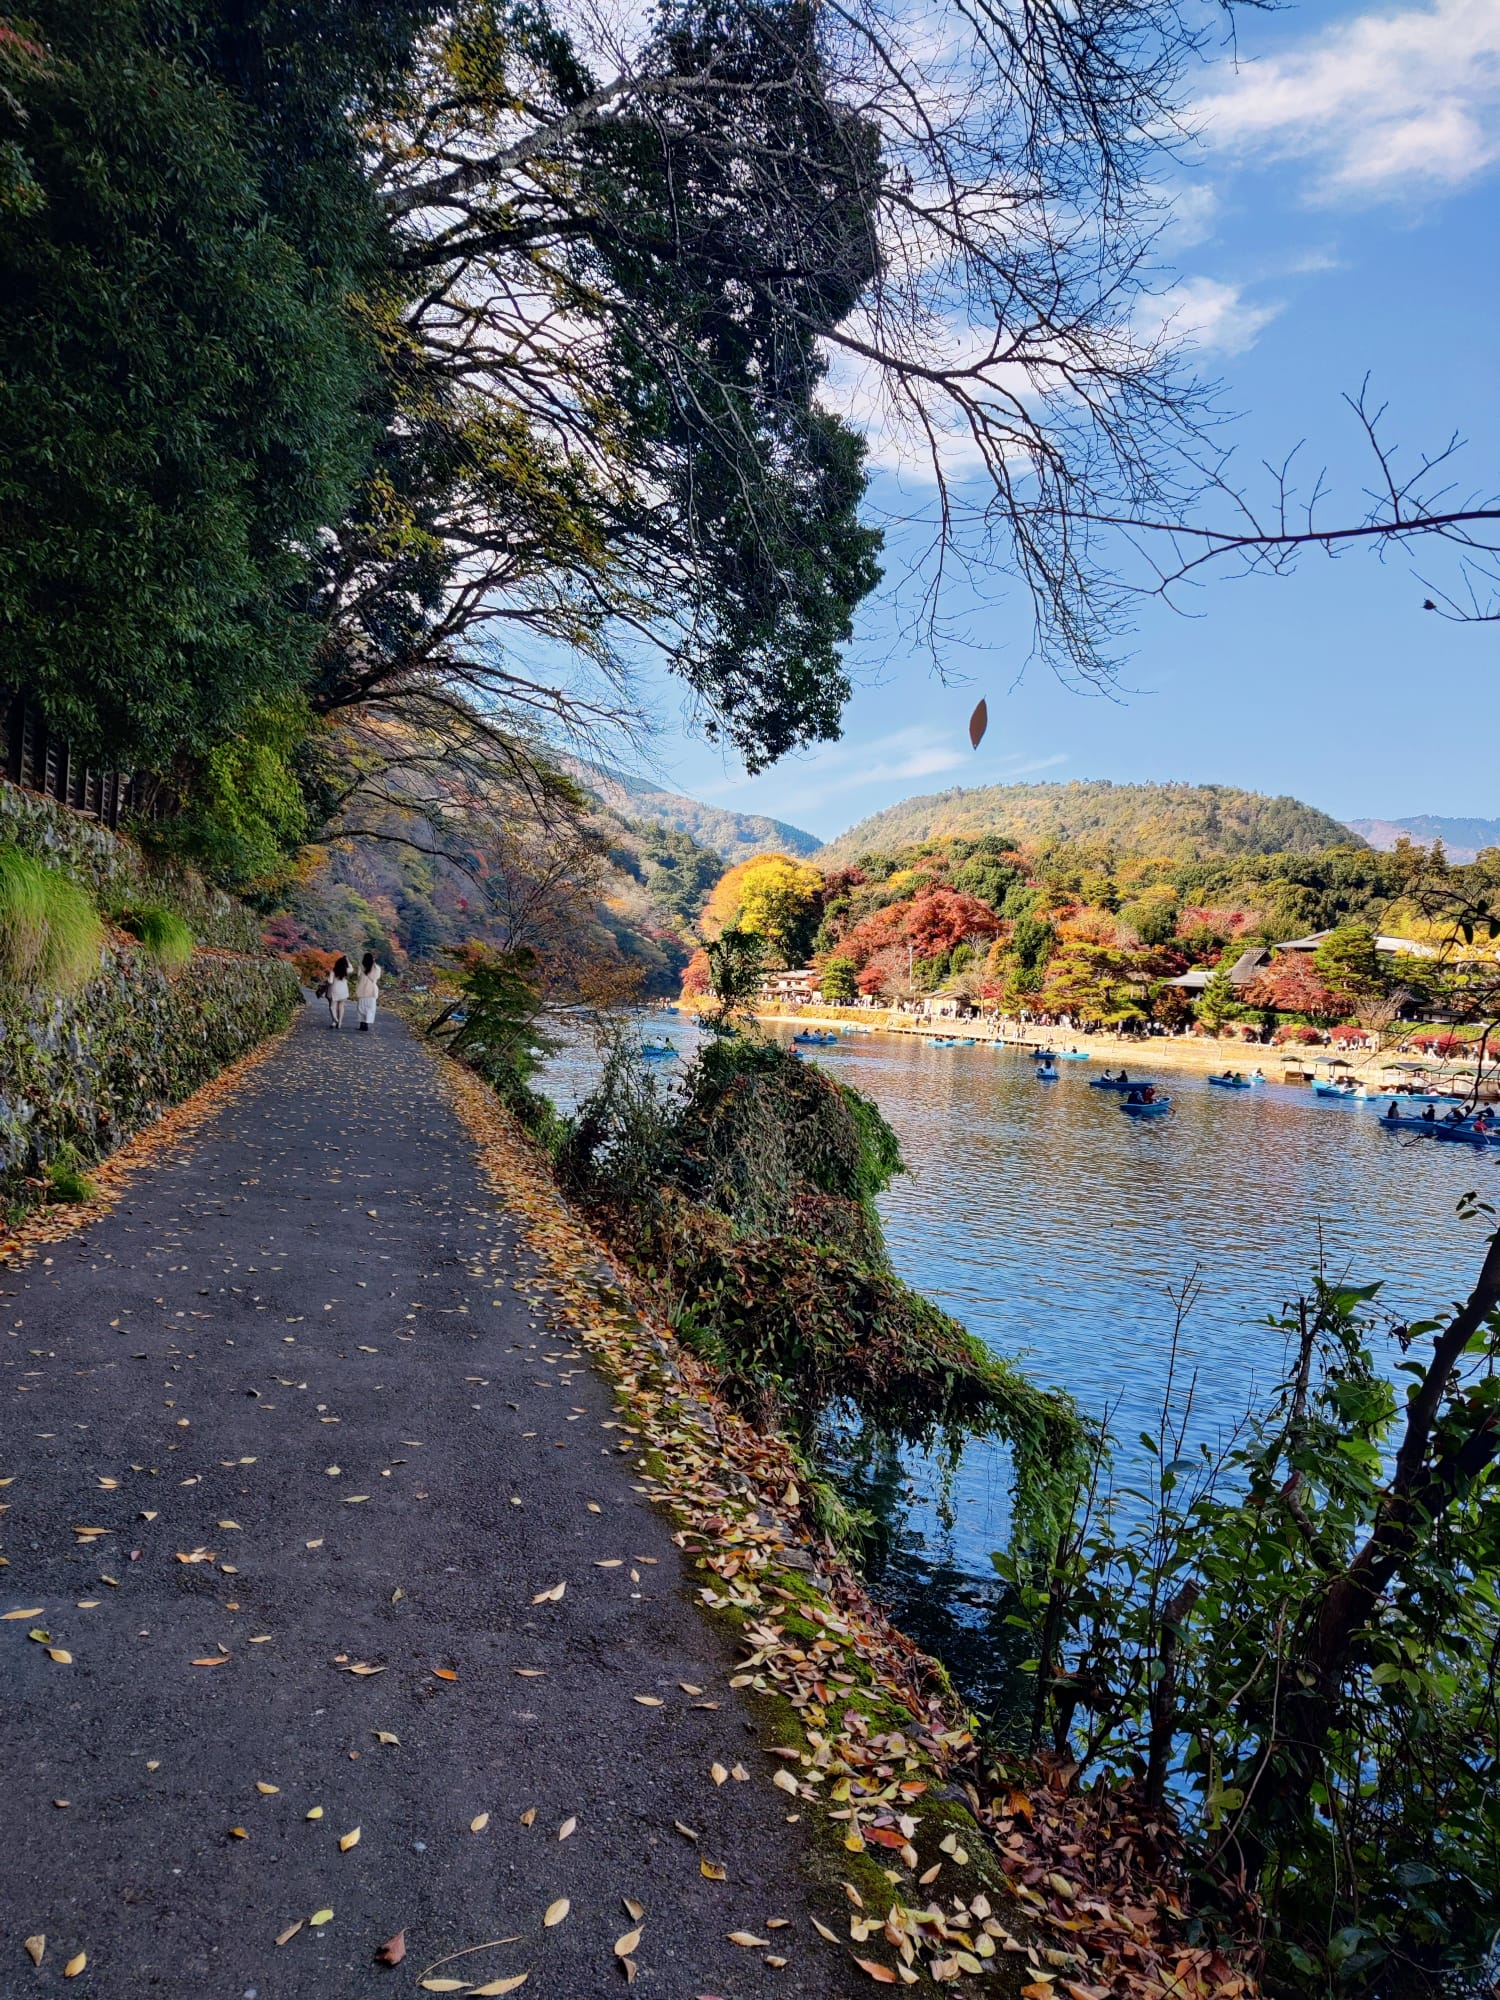
\includegraphics[height=0.5\textheight]{images/IMG-20231124-WA0038.jpg}
				\end{flushright}
				\vspace{-1cm}
				\begin{flushleft}
					\includegraphics[height=0.3\textheight]{images/DSC00708.JPG}
				\end{flushleft}}
			\only<5>{
				\includegraphics[height=0.3\textheight]{images/DSC08658.JPG}
				\vspace{-2cm}
				\begin{flushright}
					\includegraphics[height=0.5\textheight]{images/IMG_20220921_181918.jpg}
				\end{flushright}
				\vspace{-2cm}
				\begin{flushleft}
					\includegraphics[height=0.3\textheight]{images/DSC03182.JPG}
				\end{flushleft}}
			\only<6>{
				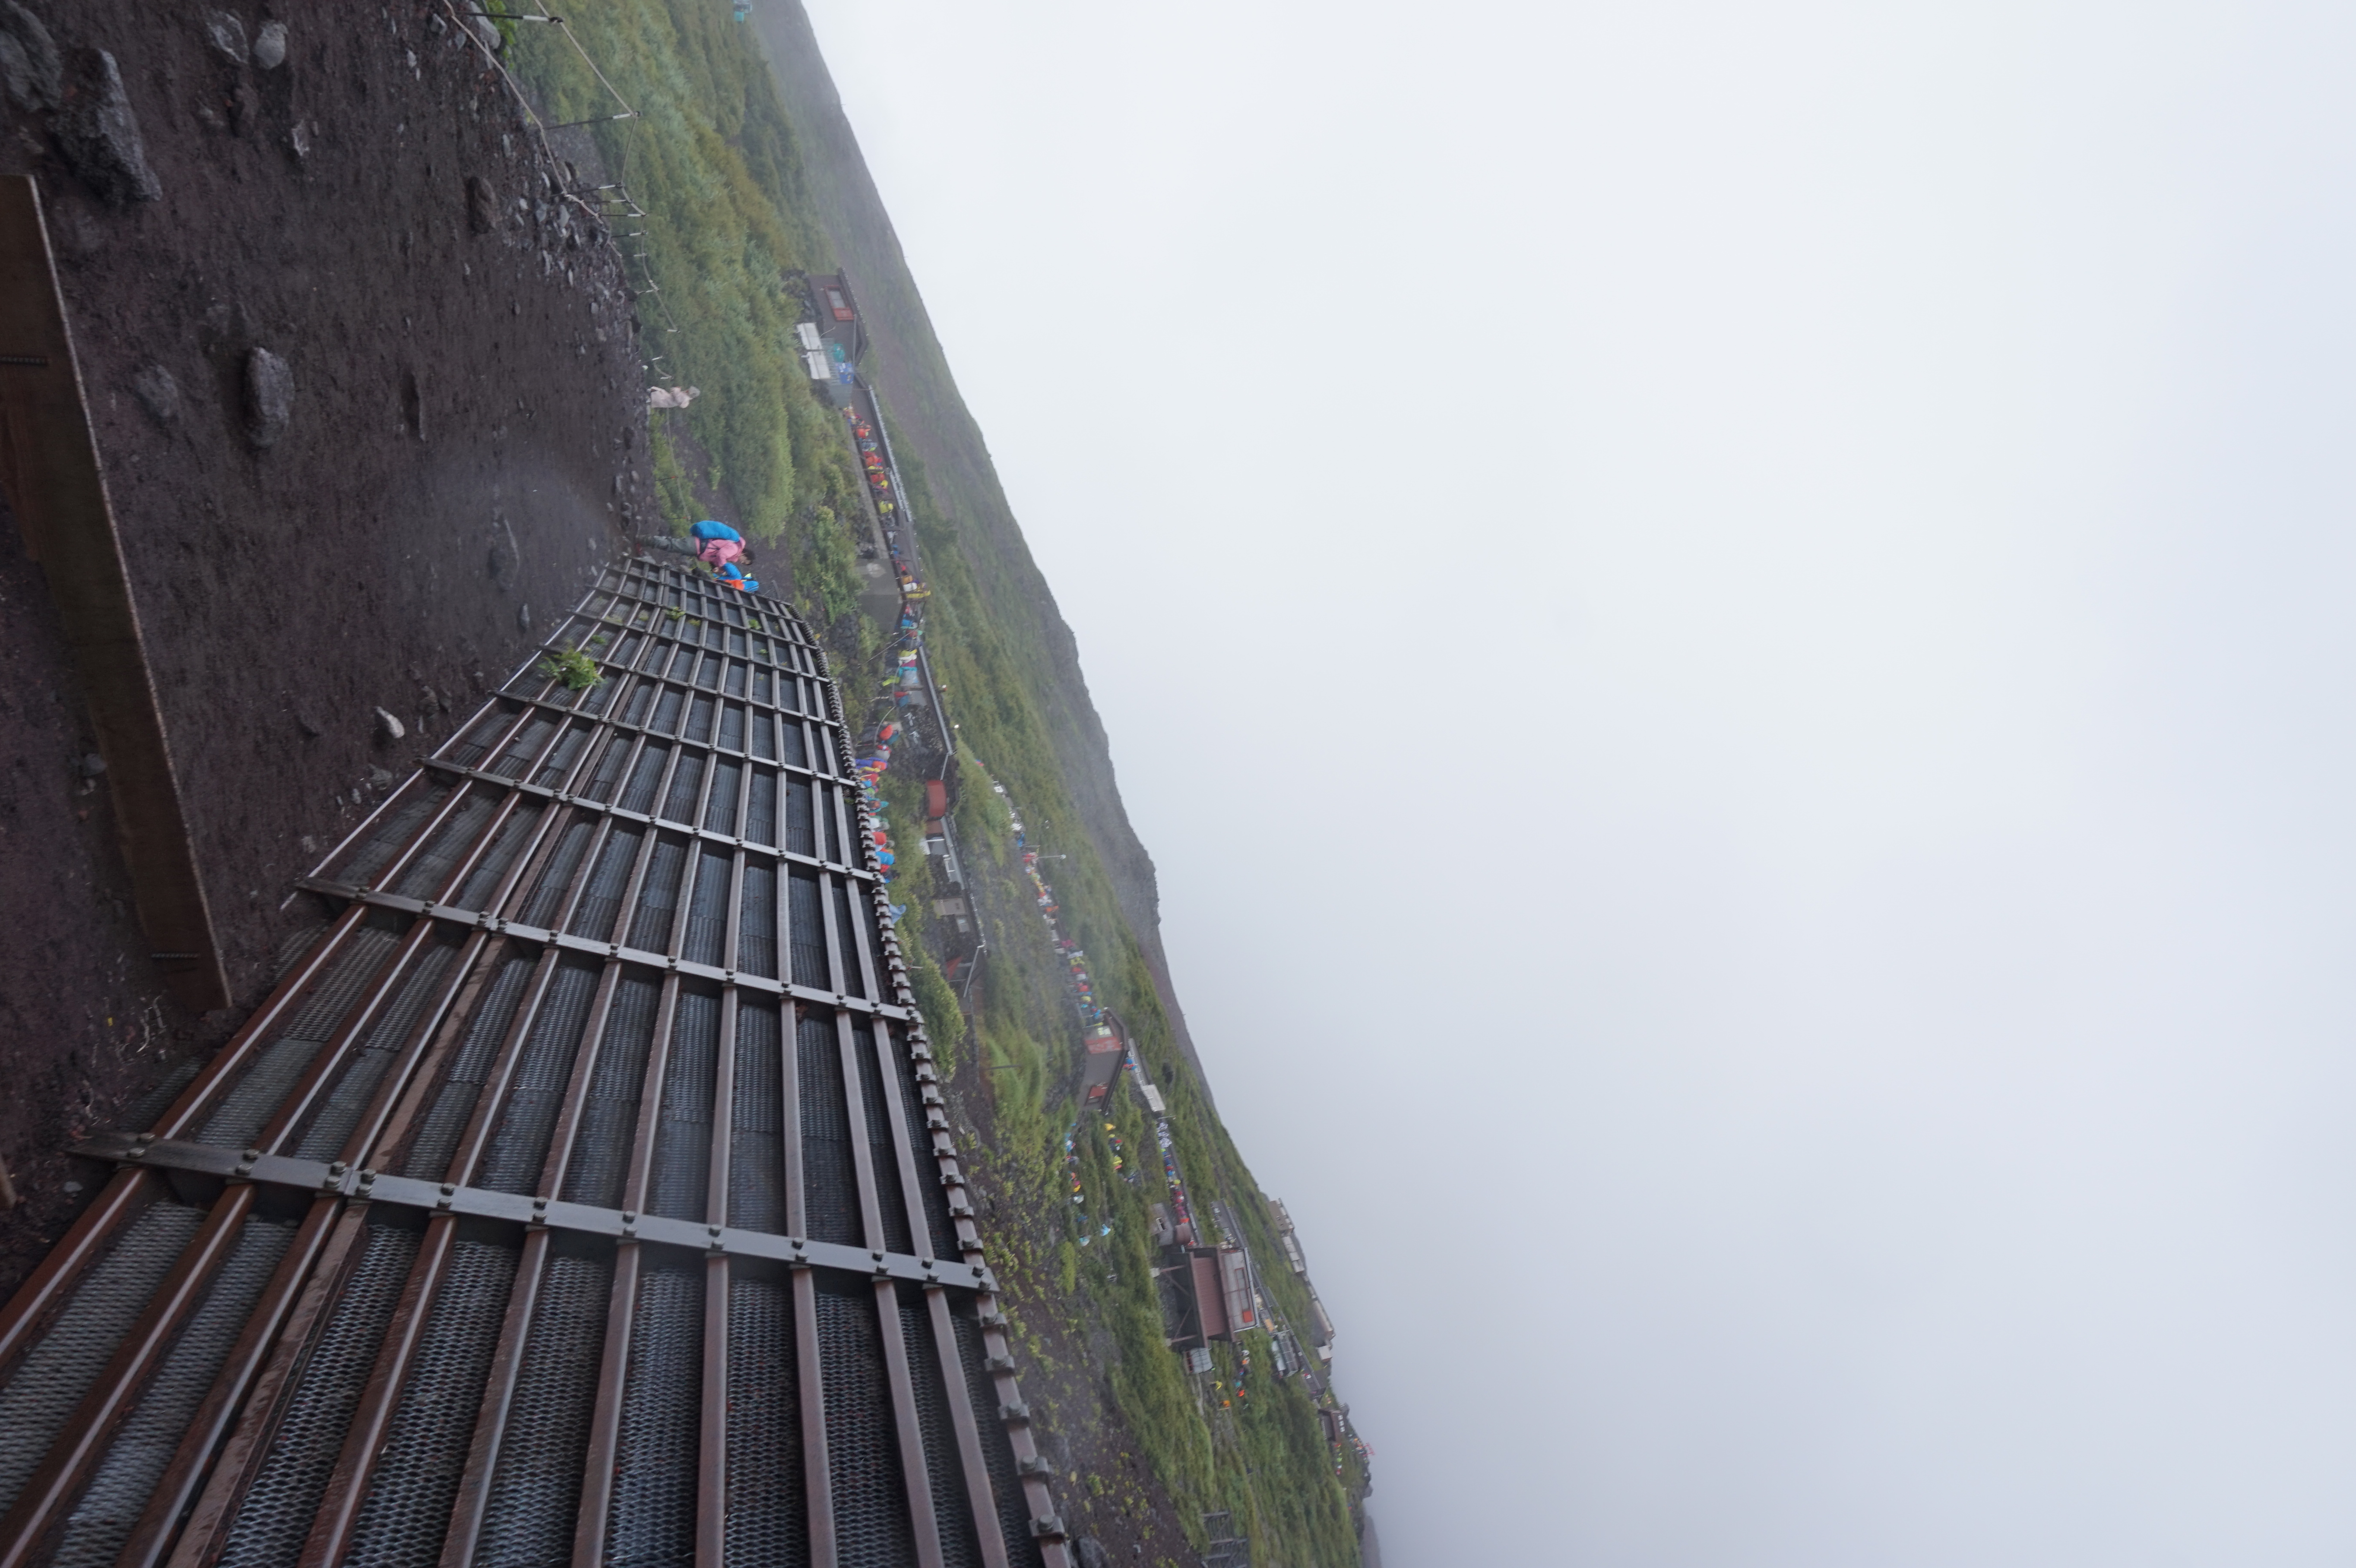
\includegraphics[height=0.3\textheight, angle=90]{images/DSC00758.JPG}
				\vspace{-3cm}
				\begin{flushright}
					\includegraphics[height=0.3\textheight]{images/DSC08658.JPG}
				\end{flushright}
%				\vspace{0.5cm}
				\begin{flushleft}
					\includegraphics[height=0.3\textheight]{images/DSC03182.JPG}
				\end{flushleft}}
			\only<7>{
				\includegraphics[height=0.3\textheight]{images/DSC03653.JPG}
				\vspace{-3cm}
				\begin{flushright}
					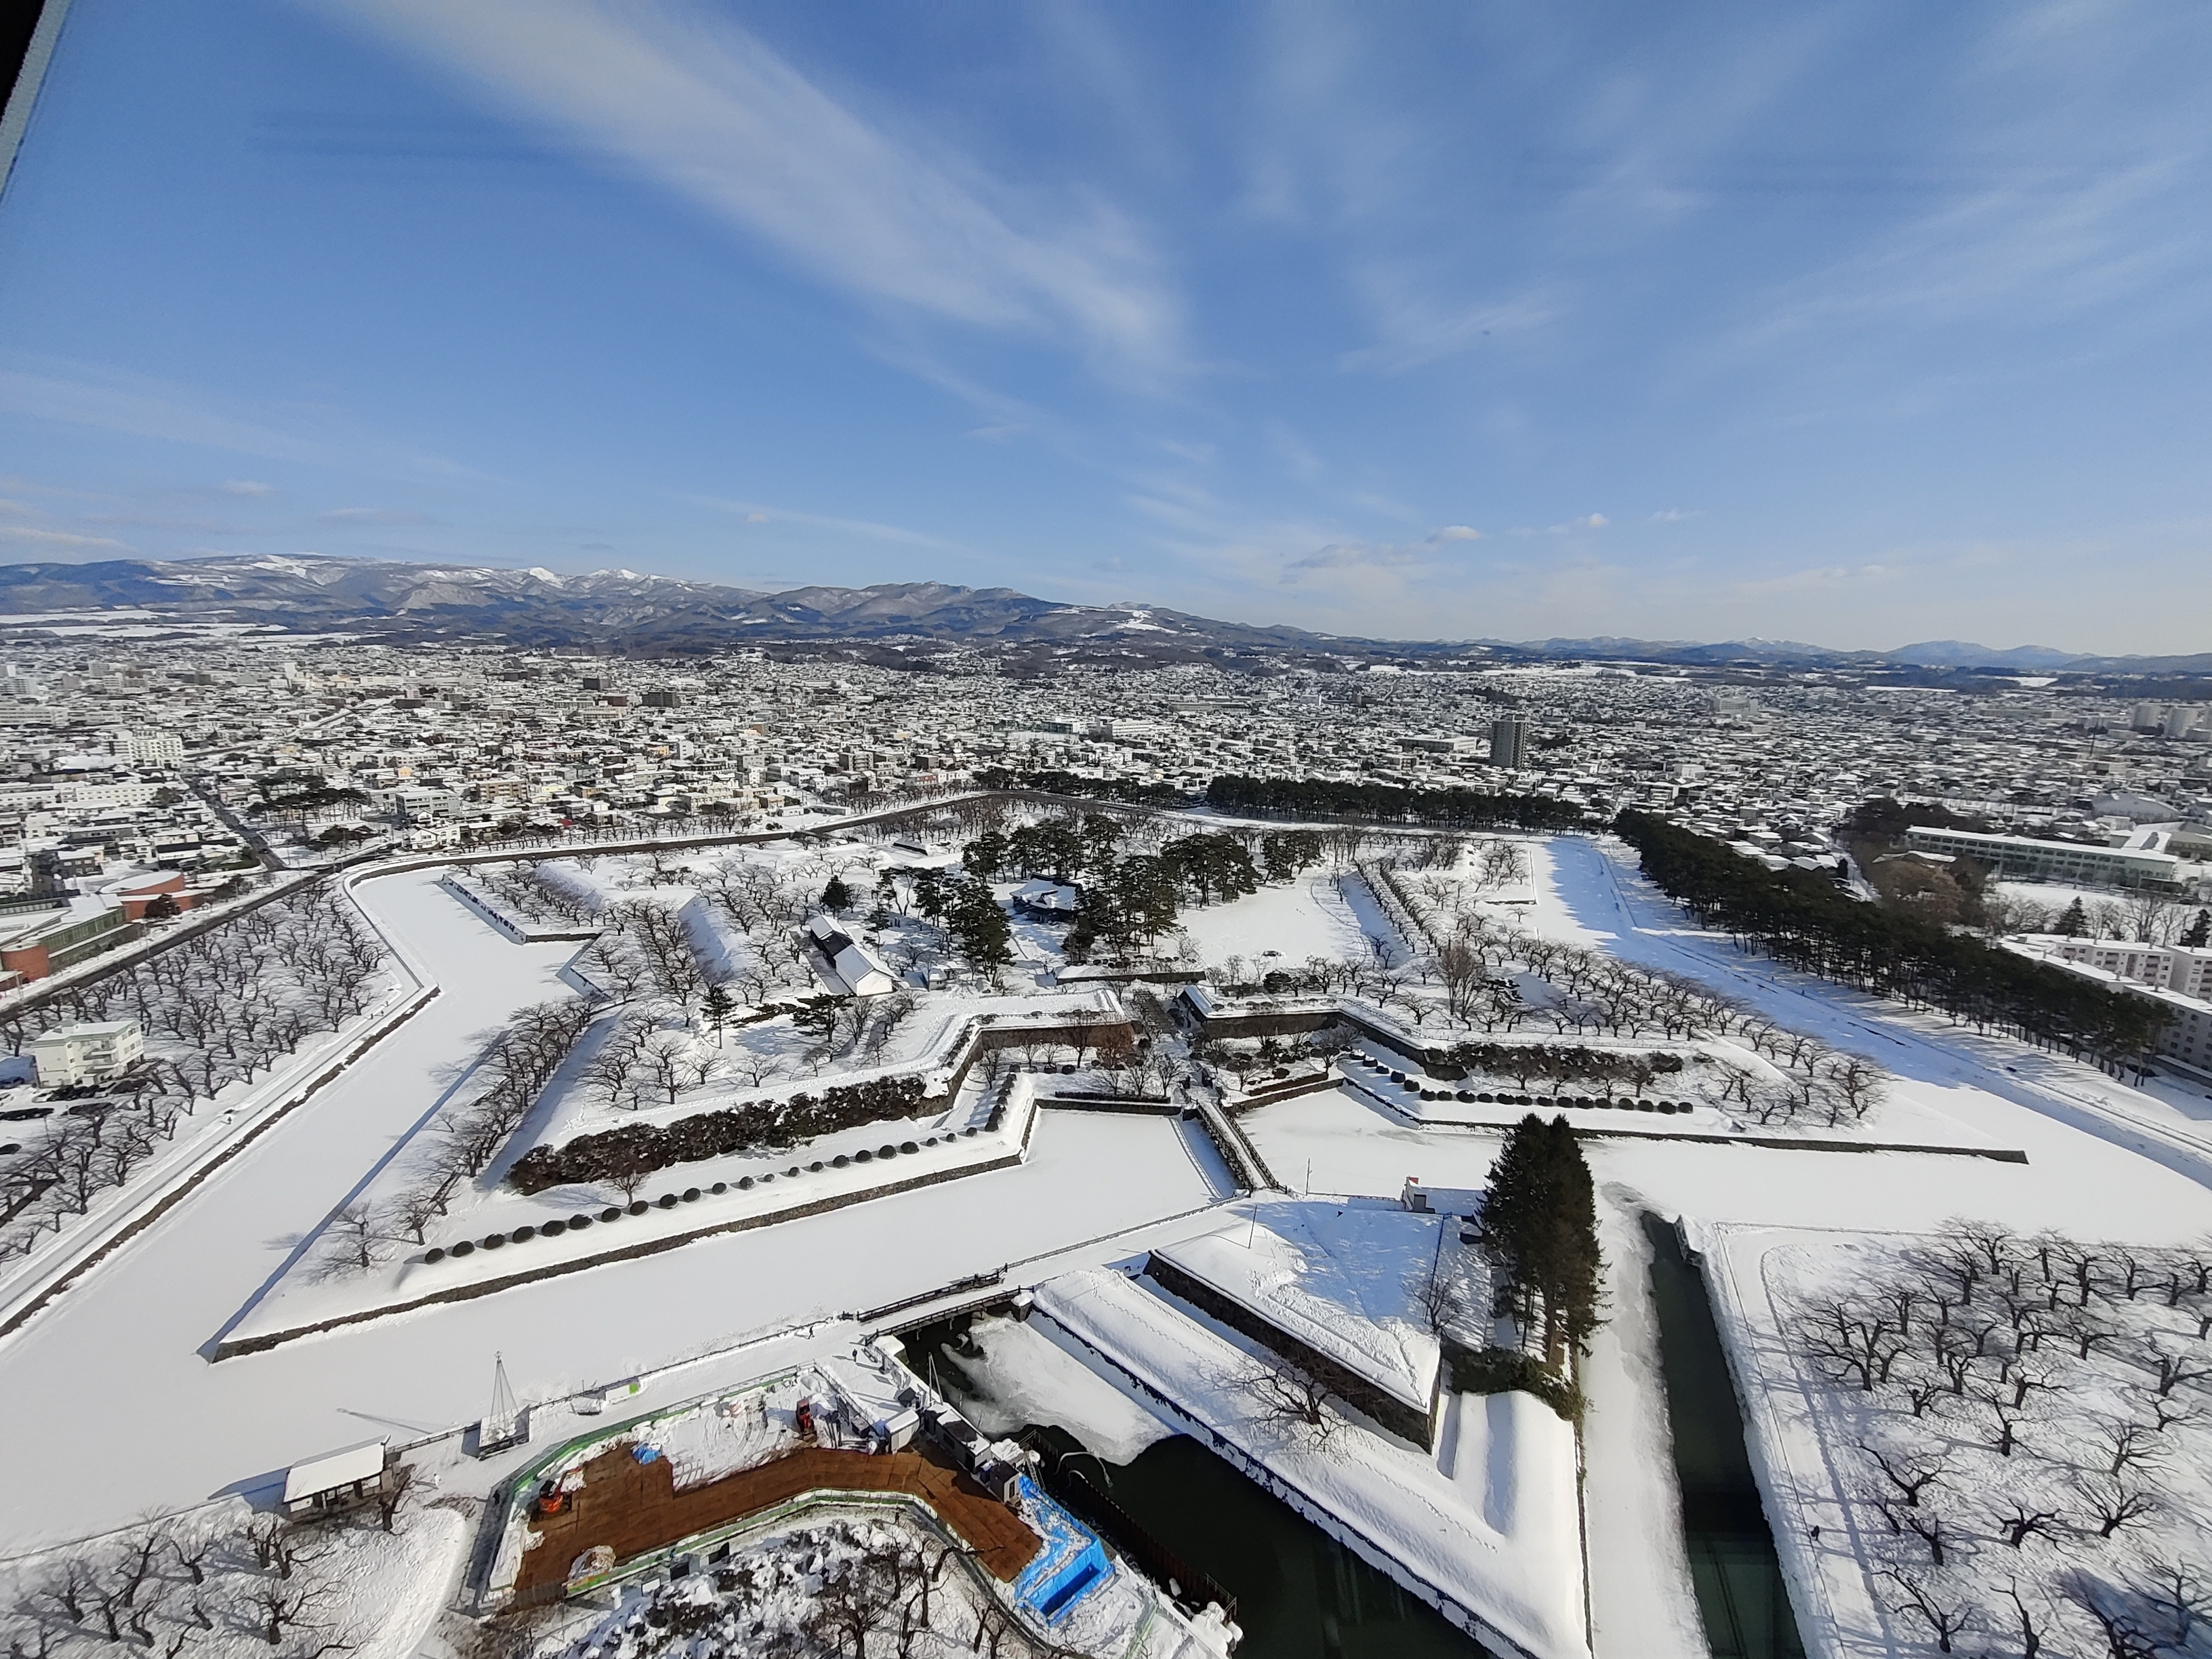
\includegraphics[height=0.3\textheight]{images/IMG_20230208_095155.jpg}
				\end{flushright}
				\vspace{0.5cm}
				\begin{flushleft}
					\includegraphics[height=0.3\textheight]{images/IMG_20221008_161529.jpg}
				\end{flushleft}
				\vspace{-3cm}
				\begin{flushright}
					\includegraphics[height=0.3\textheight]{images/IMG_20220913_171859.jpg}
				\end{flushright}}
			\only<8>{
			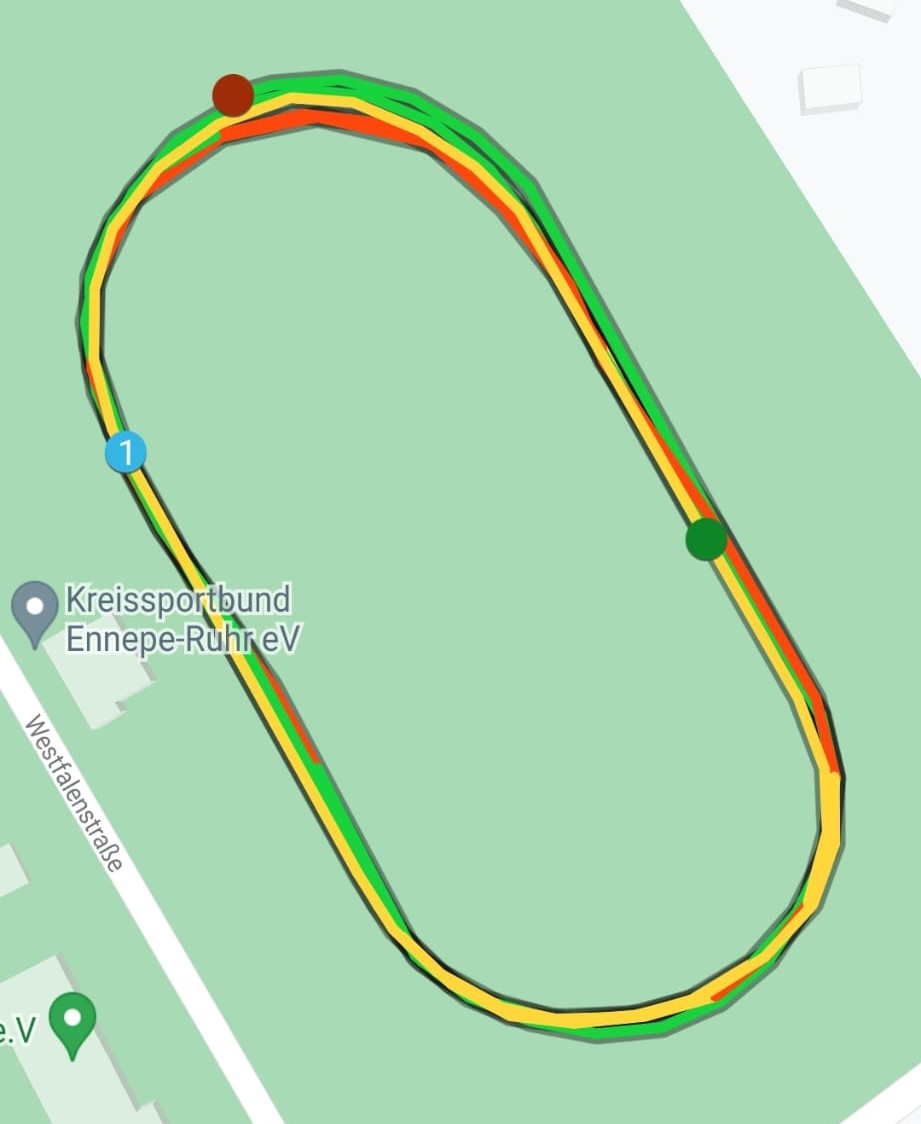
\includegraphics[height=0.4\textheight]{images/laufstrecke_rund.jpg}
			\vspace{-3cm}
				\begin{flushright}
					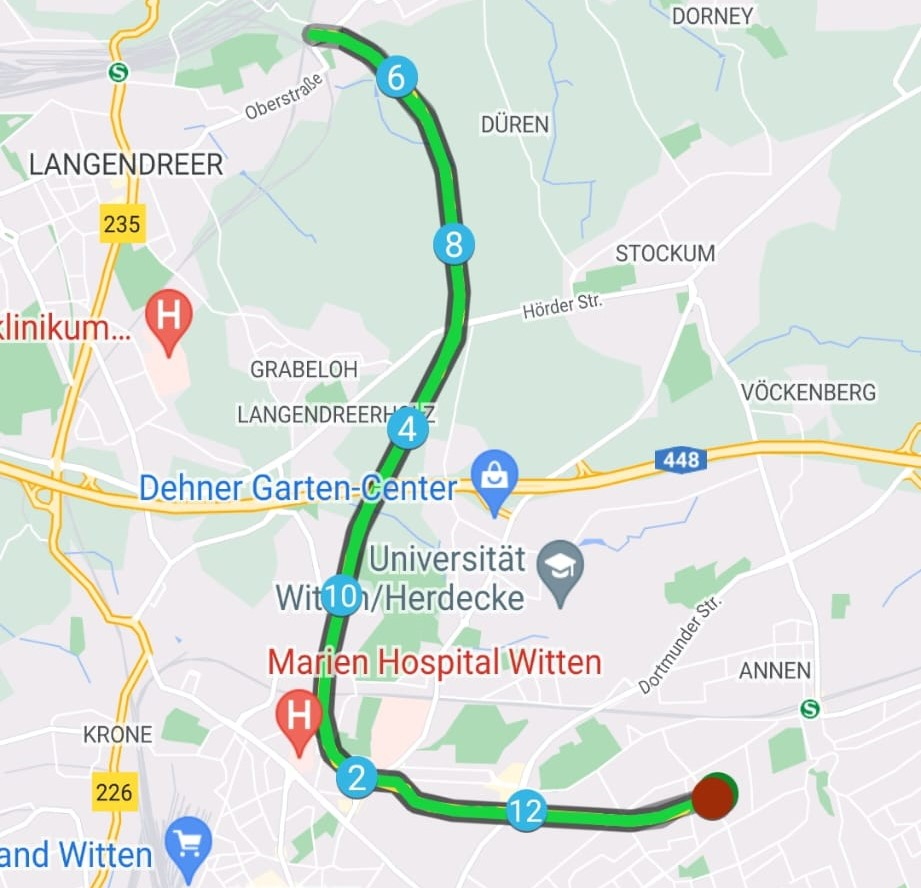
\includegraphics[height=0.4\textheight]{images/laufstecke_uturn.jpg}
				\end{flushright}
				%				\vspace{0.5cm}
				\begin{flushleft}
					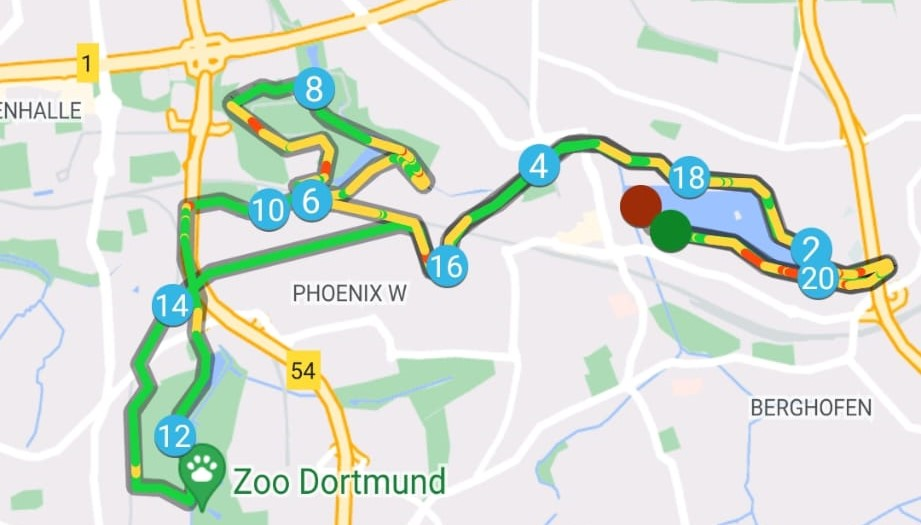
\includegraphics[height=0.3\textheight]{images/laufstrecke_komplex.jpg}
				\end{flushleft}}
		\end{minipage}
 	\end{frame}
	
	\begin{frame}{Tour4Me Demo}
	\centering
	\vspace{2cm}
	\Huge \href{http://tour4me.cs.tu-dortmund.de/} {Tour4Me}
	\end{frame}
	
	\section{Ziel}
	\begin{frame}
		\vspace{0.25cm}
		Was ist das Ziel?
		\pause
		\begin{itemize}[<+->]
			\item Grundlage: Tour4Me
			\item App erweitern und nutzbarer machen
		\end{itemize}
		\uncover<3->{
			\begin{minipage}[t][3.8cm][b]{0.48\linewidth}
				\only<4-10>{
				\begin{block}{ Mögliche algorithmische Erweiterungen: Metaheuristiken}		
					\pause			
					\begin{itemize}[<+->]
						\item AntColony
						\item Simulated Annealing
						\item Genetisch
						\item Kombinationen
					\end{itemize}
				\end{block}}
			\only<4-10>{\textcolor{white}{a}}
			\only<11>{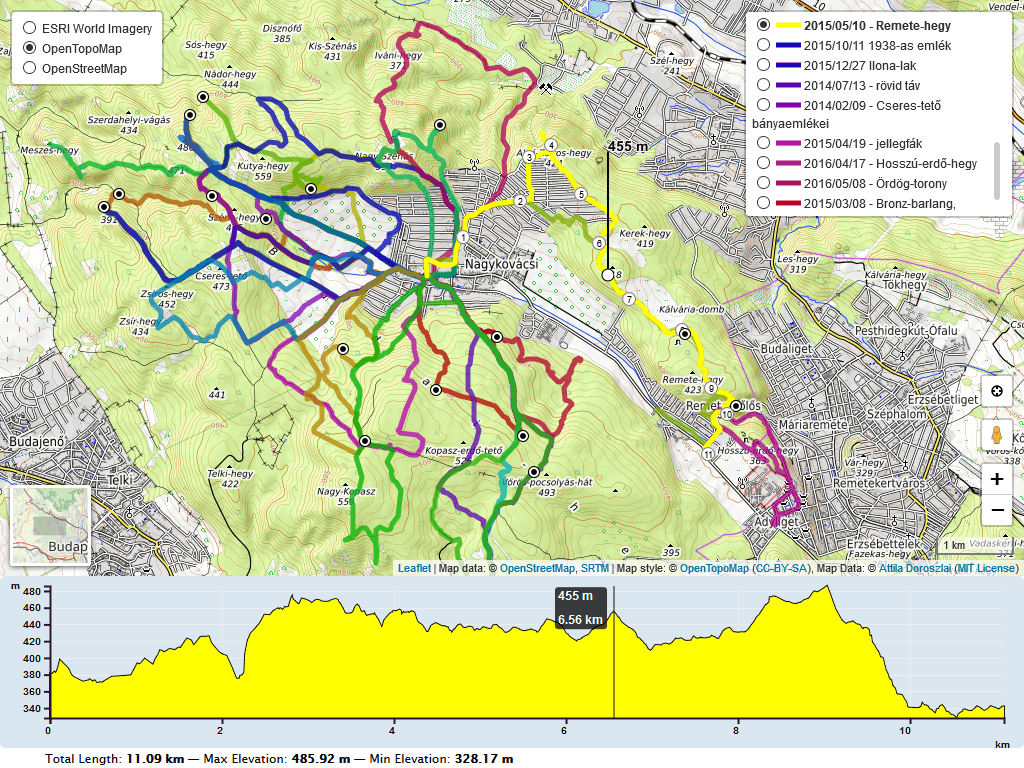
\includegraphics[height=0.5\textheight]{images/GUIIllustration.png}\footnote[frame]{https://github.com/Raruto/leaflet-elevation}}
			\only<12>{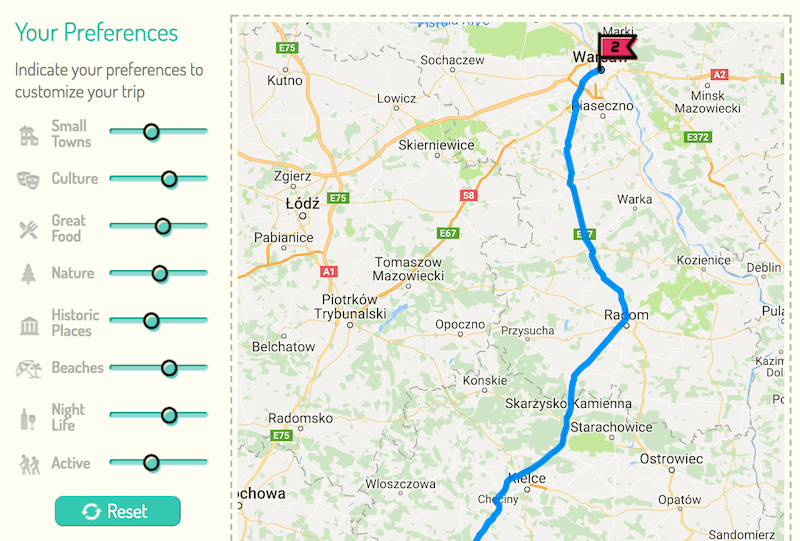
\includegraphics[height=0.5\textheight]{images/GUISliderIlustration.png}\footnote[frame]{https://www.smashingmagazine.com/2017/07/designing-perfect-slider/}}
			\only<13->{
				\begin{block}{ Mögliche algorithmische Erweiterungen: Metaheuristiken}			
					\begin{itemize}
						\item AntColony
						\item Simulated Annealing
						\item Genetisch
						\item Kombinationen
					\end{itemize}
			\end{block}
			\textcolor{white}{a}}
			\end{minipage}
			\hfill
			\begin{minipage}[t][3.8cm][b]{0.48\linewidth}
				\only<5>{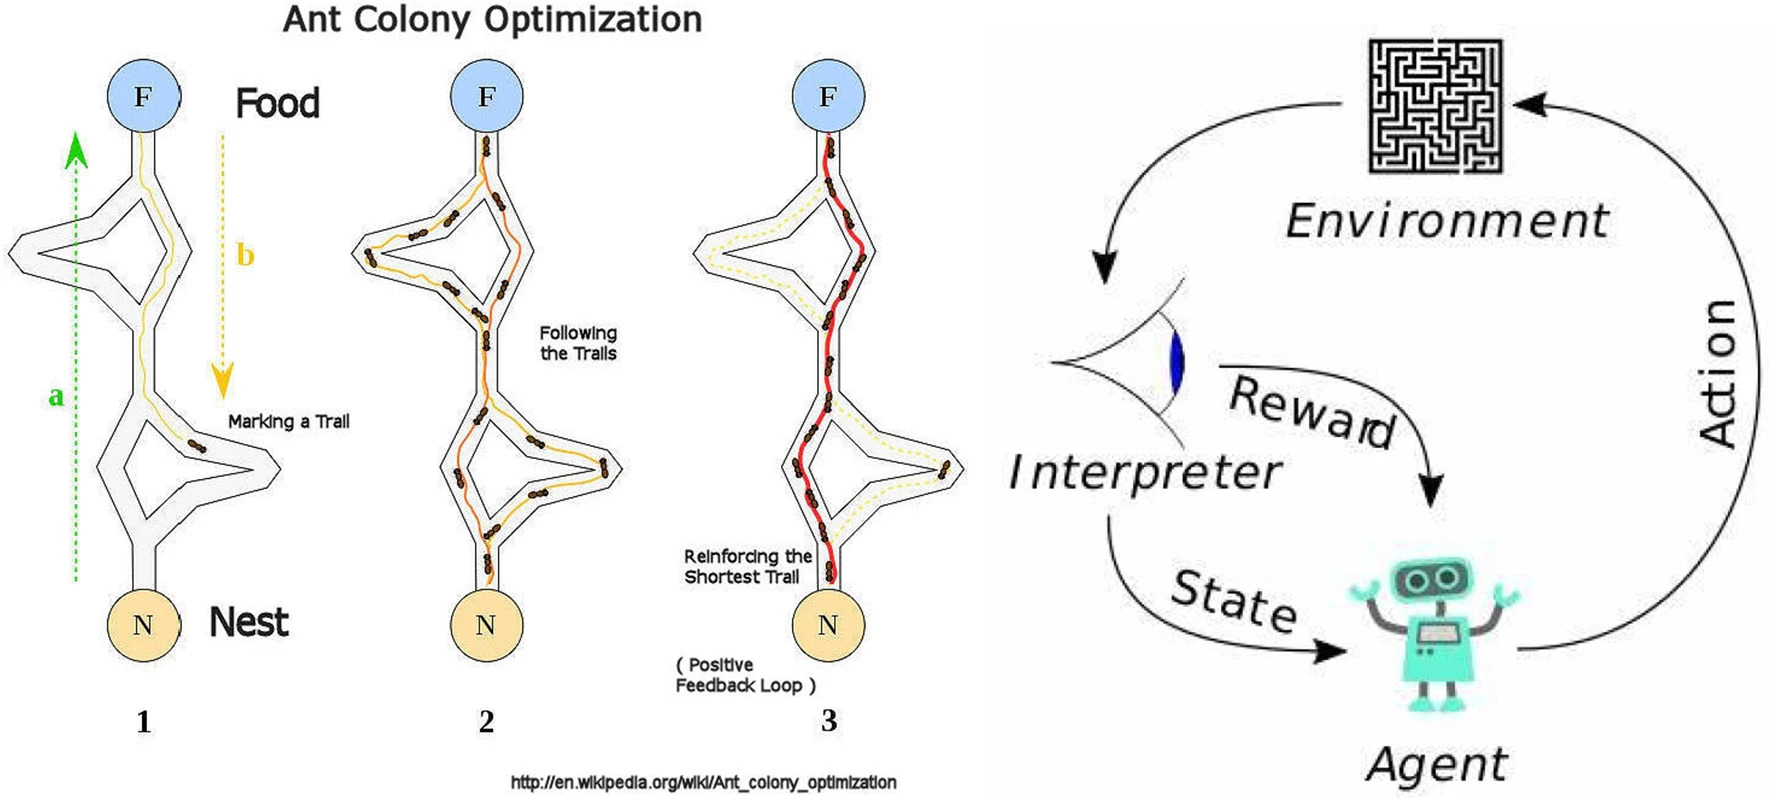
\includegraphics[height=0.35\textheight]{images/antColonyIllustration.png}\cite{liuImprovingAntColony2021}}
				\only<6>{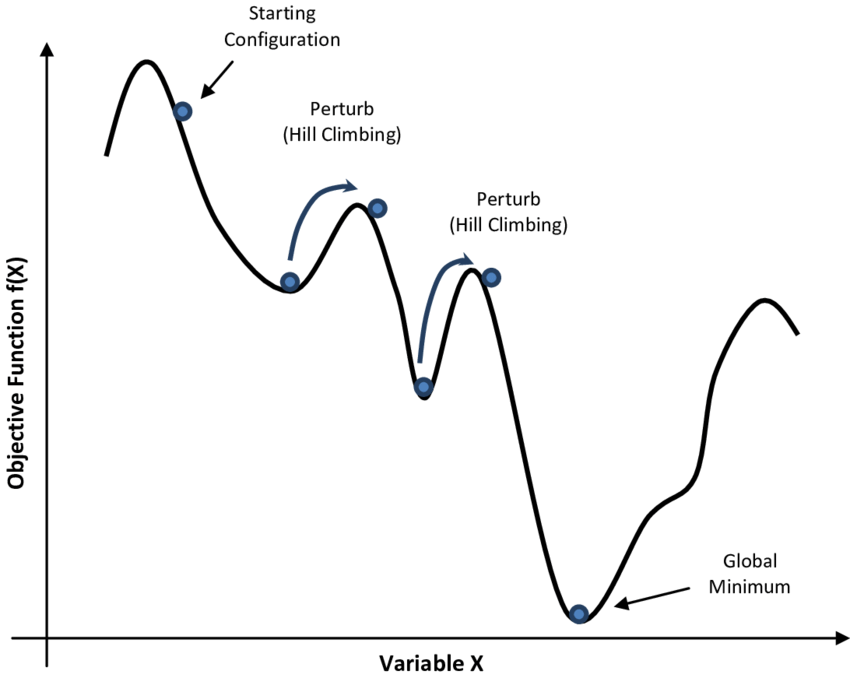
\includegraphics[height=0.5\textheight]{images/SimulatedAnnealingIllustration.png}\footnote[frame]{https://www.researchgate.net/figure/Simulated-Annealing-optimization-of-a-one-dimensional-objective-function\_fig1\_308786233}}
				\only<7>{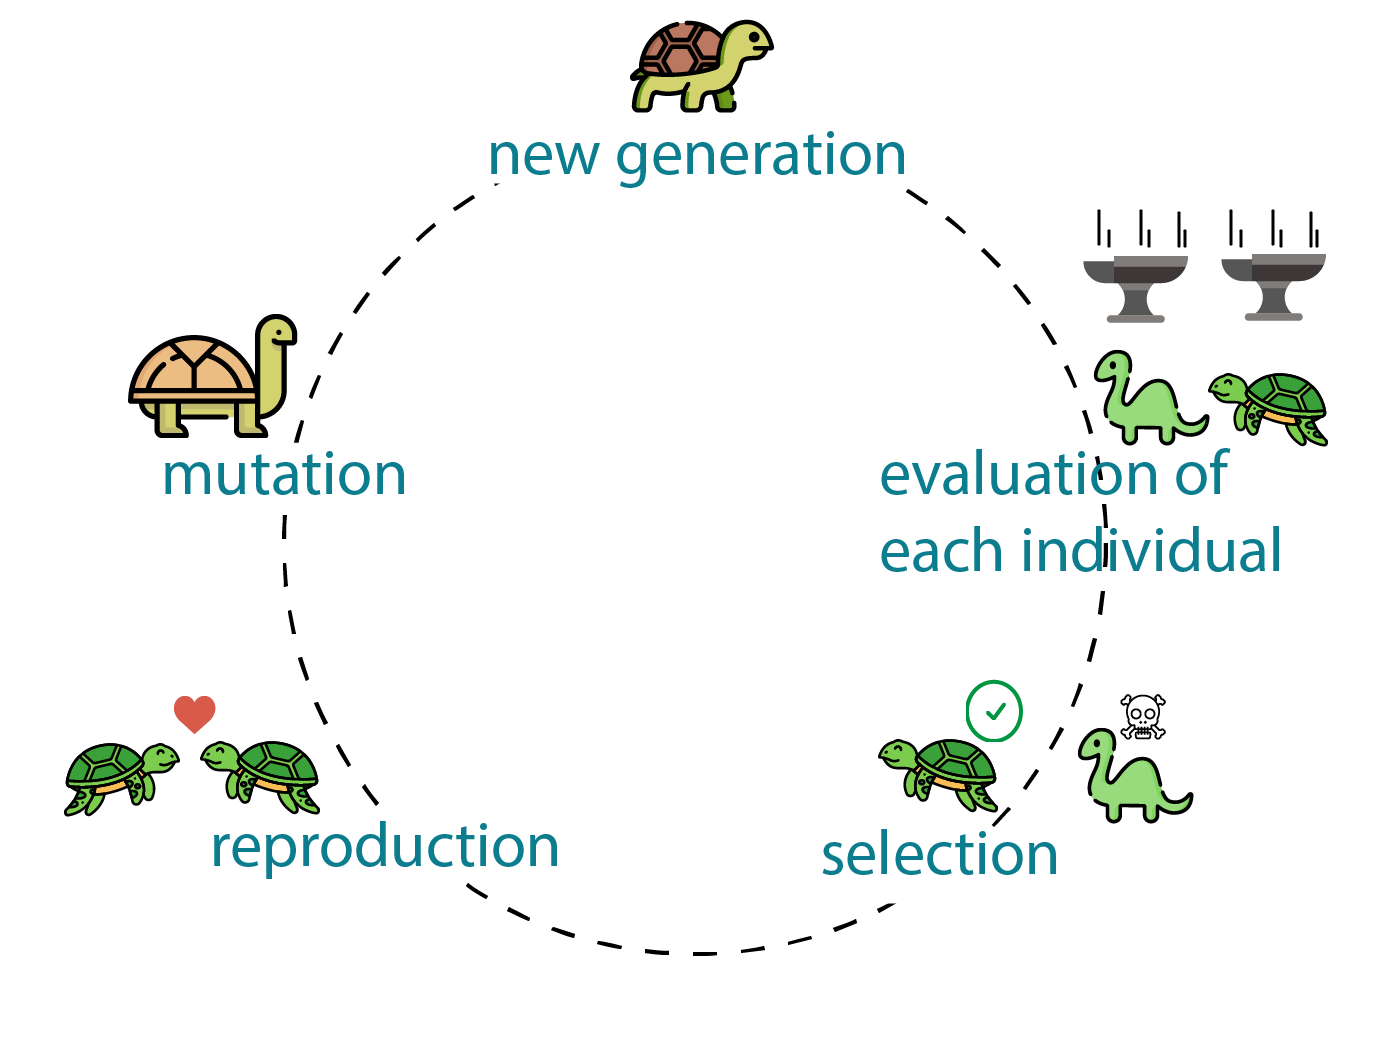
\includegraphics[height=0.5\textheight]{images/geneticAlgorithmIllustration'.png}\footnote[frame]{https://www.generativedesign.org/02-deeper-dive/02-04\_genetic-algorithms/02-04-01\_what-is-a-genetic-algorithm}}
				\only<9->{
				\begin{block}{Mögliche UI Erweiterungen: Mehr Parameter, Änderung des Interfaces}
					\pause
					\begin{itemize}
						\item<10-> Einbeziehen der genannten Faktoren
						\item<11-> Algorithmisch und in der GUI
						\item<12-> Anpassen der GUI auf neue Optionen
					\end{itemize}
				\end{block}
			\textcolor{white}{a}\\
			\textcolor{white}{a}}
			\end{minipage}}
		\only<14->{$\Rightarrow$ Allgemein: Tour4Me so anpassen, dass für (fast) jeden Startpunkt und jede Routenlänge ein (möglichst gutes) Ergebnis ausgegeben wird}
	\end{frame}
	
	
	\section{Motivation und Hintergrund}	
	\begin{frame}
		\vspace{0.5cm}
		Viele Algorithmen, Ansätze und viel  Forschung zu Kürzeste-Wege-Problemen
		\pause
		\begin{itemize}[<+->]
			\item Reviews, Vergleiche und Analysen \cite{madkourSurveyShortestPathAlgorithms2017, sommerShortestpathQueriesStatic2014, wayahdiGreedyAStarDijkstra2021}
			\item Zusätzlich weitere heuristische Ansätze
			\begin{itemize}[<+->]
				\item Local Search Varianten \cite{braysyVehicleRoutingProblem2005, irnichSequentialSearchIts2006, ropkeHeuristicExactAlgorithms2005}
				\item Neighborhood basierte Ideen \cite{braysyVehicleRoutingProblem2005, irnichSequentialSearchIts2006, ropkeHeuristicExactAlgorithms2005}
			\end{itemize} 
		\item Algorithmische Routing-Probleme  bereits NP-schwer \cite{reineltTravelingSalesmanComputational2003}
		\begin{itemize}[<+->]
			\item Traveling Salesman (TSP)\cite{gendreauHandbookMetaheuristics2010} 
			\item Vehicle routing \cite{braysyVehicleRoutingProblem2005, irnichSequentialSearchIts2006}
		\end{itemize}
		\end{itemize}
		\pause
		
		$\Rightarrow$ Rundtrips mit Nebenbedingungen noch komplexer \cite{gemsaEfficientComputationJogging2013}
		\pause
		\begin{itemize}[<+->]
			\item Vorhandene Tools meist eingeschränkt
			\item Auswahl an Nebenbedingungen beschränkt
			\item Editieren schwierig/ ignoriert Nebenbedingungen
		\end{itemize}
	\end{frame}
	
	\begin{frame}{Beispiele}
		\centering
		\vspace{2.5cm}
		\Huge
		\only<1> {\href{https://www.routeyou.com}{RouteYou}}
		\only<2> {\href{https://www.routeloops.com/}{RouteLoops}}
	\end{frame}
	
	
	\section{Vorgehensweise}		
	\begin{frame}	
		\vspace{0.5cm}
		\begin{block}{Was wird gemacht?}
			\pause
			\begin{itemize}[<+->]
				\item Interface zum Testen neuer Ansätze und Metaheuristiken (C\#)
				\item Einbauen neuer Auswahloptionen für User (z.B. Höhe/Anstieg)
				\item Implementieren verschiedener Ansätze
				\begin{itemize}[<+->]
					\item Metaheuristiken
					\item Kombinationen dieser
					\item Kobination mit bereits implementierten Ansätzen
				\end{itemize}
				\item Auswertung und Vergleich der Ansätze
				\item Anpassen des User Interfaces
				\item Auswahl des/der best passenden Umsetzungen
				\item Übertragen in eine finale Tour4Me Anwendung (vollständig c++ oder C\#)
			\end{itemize}
		\end{block}
	\end{frame}
	
%	\begin{frame}{Timeline}
%		\centering
%		\vspace{0.5cm}
%		\tikzstyle{descript} = [text = black,align=center, minimum height=1.8cm, align=center, outer sep=0pt,font = \footnotesize]
%		\begin{tikzpicture}[very thick, black, scale=0.9, font=\scriptsize]
%			\small
%			
%			%% Coordinates
%			\coordinate (S) at (-3,0);
%			\coordinate (O) at (-1,0); % Origin
%			\coordinate (P1) at (1,0);
%			\coordinate (P2) at (8,0);
%			\coordinate (P3) at (11,0);
%			\coordinate (P4) at (12.5,0);
%			\coordinate (F) at (13,0); %End
%			\coordinate (E1) at (5,0); %Event
%			\coordinate (E2) at (0.5,0); %Event
%			
%			
%			%% Arrow
%			\draw[->] ($(S)+(0,-0.1)$) -- ($(F)+(0,-0.1)$);
%			%% Ticks
%			\foreach \x in {-2,0,2,...,12}
%			\draw(\x cm,6pt) -- (\x cm,-6pt);
%			%% Labels
%			\foreach \i \j in {-2/Nov, 0/Dez,2/Jan,4/Feb,6/Mär,8/Apr,10/Mai,12/Jun}{
%				\draw (\i,-0.1) node[below=3pt] {\j} ;
%			}
%			\pause
%			
%			%% Filled regions
%			\fill[color=ColorOne!20] rectangle ($(S)+(0.2,0)$) -- (P1) -- ($(P1)+(0,1)$) -- ($(S)+(0.2,1)$);
%			\path [pattern color=ColorOne!80, pattern=north east lines, line width = 1pt, very thick] rectangle ($(O)+(0.6,0)$) -- ($(O)+(2,0)$) -- ($(O)+(2,1)$) -- ($(O)+(0.6,1)$);
%			\draw ($(O)+(-0.4,0.5)$) node[activity,ColorOne] {Vorarbeit};
%			\pause	
%			
%			%% Description
%			\node[descript,fill=ColorOne!15,text=ColorOne](P0) at ($(O)+(2,-2.5)$) {%
%				Literatur\\
%				Beispiele\\
%				Erste Implementierung Interface};
%			
%			%% Arrows
%			\path[->,color=ColorOne] ($(O)+(-0.5,-0.1)$) edge [out=-90, in=130]  ($(P0)+(0,1)$);
%			\pause
%			
%			\fill[color=ColorTwo!15] rectangle (P1) -- (P2) -- ($(P2)+(0,1)$) -- ($(P1)+(0,1)$);
%			\draw ($(P2)+(-3.55,0.5)$) node[activity,ColorTwo] {Implementierung und Testen versch. Algorithmen,\\ Ändern anderer Teile der App};
%			\pause
%			
%			\fill[ColorThree!30] rectangle (P2) -- (P3) -- ($(P3)+(0,1)$) -- ($(P2)+(0,1)$);
%			\draw ($(P3)+(-1.55,0.5)$)  node[activity, ColorThree] {Ergebnisse \\sammeln};
%			\pause
%			
%			\fill[ColorFour!20] rectangle (P3) -- (P4) -- ($(P4)+(0,1)$) -- ($(P3)+(0,1)$);
%			\draw ($(P4)+(-0.8,0.5)$)  node[activity, ColorFour!80!black] {Nur noch \\schreiben};
%			\pause
%			
%			
%			%% Events
%			\draw [decorate,decoration={brace,amplitude=6pt}]($(P1)+(-1.8,1.2)$) -- ($(F)+(-0.5,1.2)$) node [black,midway,above=6pt, align=center] {Schreiben an der Masterarbeit};
%			
%			
%		\end{tikzpicture}
%	\end{frame}
%	
	
%	\section{Literatur}
	\begin{frame}[allowframebreaks]{Literatur}
		
		\bibliography{LS11Buchin.bib}
	\end{frame}
	
	
\end{document}

